\chapter{Trabalho Futuros} % (fold)
\label{cha:trabalho_futuros}

Este trabalho será segmentado cronologicamente nas seguintes etapas:

\begin{enumerate}

    \item \textbf{Implementação de Técnicas de Planejamento}:\\
        Deseja-se obter os melhores trajetos a serem percorridos pelo objeto até sua pose final. Inicialmente as seguintes técnicas serão implementadas e avaliadas:
            \begin{enumerate}
                \item Discretização do ambiente:
                    \begin{enumerate}
                        \item Mapa Discreto com células fixas;
                        \item Mapa Discreto com células de tamanho variável.
                    \end{enumerate}
                \item Busca pelos Caminhos:
                    \begin{enumerate}
                        \item Métodos Exatos:
                            \begin{enumerate}
                                \item Dijkstra.
                                \item $A^{*}$;
                            \end{enumerate}
                        \item Métodos Probabilísticos:
                            \begin{enumerate}
                                \item RRT.
                            \end{enumerate}
                    \end{enumerate}
            \end{enumerate}

    \item \textbf{Modelagem da Função de Custo}\\
    A função que descreve o gasto relacionado a certo trecho do caminho proposto como resultado do Problema de Planejamento do Objeto (Problema 1). Baseado nesta função, será possível selecionar os agentes mais aptos dentre os quais são capazes de realizar o transporte nas determinadas etapas do caminho.

    Serão realizados diversos experimentos variando o tipo de custo associado a cada trecho. Esta variação tem seu objetivo na formulação da função que melhor descreve o custo. Serão considerados:
        \begin{enumerate}
            \item Tempo necessário para o trecho;
            \item Distância: Euclidiana, Euclidiana Quadrática, Manhattan, Distância em Grafo;
            \item Gasto energético: Deslocamento, Decolagem, Aterrissagem.
        \end{enumerate}

    \item \textbf{Alocar tarefa baseado na Função de Custo}\\
    Considerando o custo associado a cada trecho do percurso do objeto, realizar a distribuição da tarefa de transporte aos agentes que melhor atenderem às necessidades do mesmo. Serão consideradas as seguintes regras para a alocação de tarefa, na seguinte ordem:
        \begin{enumerate}
            \item Proximidade do local da Tarefa: aloca a atividade para o agente mais próximo à localidade de realização da mesma;
            \item Robô livre: atribui a tarefa ao primeiro agente que estiver em espera;
            \item Leilão: realizar um passo de anúncio da tarefa e alocar para o agente com o melhor lance.
        \end{enumerate}

    \item \textbf{Implementação de Técnicas de Coordenação}\\
    Realizar o controle da equipe de agentes utilizando técnicas diversas para a mesma tarefa. Uma comparação entre o desempenho em relação a tempo e custo computacional deve guiar a escolha pela melhor tática para a tarefa de transporte. Serão realizados teste com as seguintes estratégias:
        \begin{enumerate}
            \item Centralizado;
            \item \emph{AlphaBeta};
            \item Descentralizado.
        \end{enumerate}

    \item \textbf{Experimentação}\\
    Os experimentos serão realizados em ambientes simulados e reais. Será utilizado como plataforma de desenvolvimento o \emph{framework} \emph{Robot Operating System (ROS)}(\cite{ROS}), pois o mesmo provê um conjunto de sistemas amplamente utilizado no desenvolvimento de sistemas autônomos, muitos deles já disponíveis para uso, agilizando o desenvolvimento de aplicações neste contexto.

    Experimentos simulados serão implementados nos simuladores \emph{Gazebo}(\cite{Gazebo}) e \emph{V-REP}(\cite{VREP}). As duas plataformas disponibilizam modelos de diversos agentes robóticos, além de possuir integração com o \emph{ROS}. A experimentação real se baseará no uso dos sistemas \emph{iRobot Create} e \emph{AR.Drone}, agentes terrestres e aéreos, respectivamente.

    \begin{figure}[!h]
      \centering

      % \begin{subfigure}[b]{0.48\textwidth}
      %   \centering
      %   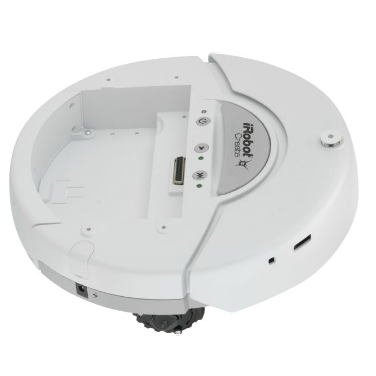
\includegraphics[width=0.7\textwidth]{img/irobot_create.jpg}
      %   \caption{iRobot Create}
      % \end{subfigure}
      % \begin{subfigure}[b]{0.48\textwidth}
      %   \centering
      %   \includegraphics[width=0.7\textwidth]{img/ar-drone.jpg}
      %   \caption{AR.Drone}
      % \end{subfigure}

      \caption{Plataformas Robóticas utilizadas na experimentação real.}
      \label{fig:robos}

    \end{figure}

    % A implementação do sistema proposto será realizada através do
    % das soluções em ambientes simulados e reais. Serão usados para formar a equipe heterogênea a plataforma iRobot Create como agente terrestre e o Quadrirotor AR.Drone como agente aéreo.

    \item \textbf{Escrita de Artigos Científicos}\\
    Pretende-se, como consequência desta pesquisa, realizar a submissão dos resultados mais relevantes para a comunidade científica no campo de coordenação de multi-agentes. As conferências alvo deste trabalho são:
        \begin{itemize}
            \item ICRA;
            \item IROS.
        \end{itemize}

    \item \textbf{Escrita da Dissertação}.
\end{enumerate}

A Tabela~\ref{table:cronograma} apresenta um cronograma das etapas mencionadas anteriormente para o período de 12 meses.

\begin{table}[h]
    \begin{tabular}{|c|c|c|c|c|c|c|c|c|c|c|c|c|}
    \hline

    \multirow{2}{*}{Atividade} & \multicolumn{6}{c|}{2014} & \multicolumn{6}{c|}{2015} \\ \cline{2-13}
    ~ & Jul    & Ago    & Set    & Out    & Nov    & Dez    & Jan & Fev & Mar & Abr & Mai & Jun \\ \hline

    1 & $\ast$ & $\ast$ & ~      & ~      & ~      & ~      & ~      & ~      & ~      & ~      & ~      & ~      \\ \hline
    2 & ~      & $\ast$ & $\ast$ & ~      & ~      & ~      & ~      & ~      & ~      & ~      & ~      & ~      \\ \hline
    3 & ~      & ~      & $\ast$ & $\ast$ & $\ast$ & ~      & ~      & ~      & ~      & ~      & ~      & ~      \\ \hline
    4 & ~      & ~      & ~      & $\ast$ & $\ast$ & $\ast$ & $\ast$ & ~      & ~      & ~      & ~      & ~      \\ \hline
    5 & ~      & ~      & $\ast$ & $\ast$ & $\ast$ & $\ast$ & $\ast$ & $\ast$ & $\ast$ & $\ast$ & ~      & ~      \\ \hline
    6 & ~      & $\ast$ & $\ast$ & ~      & ~      & ~      & $\ast$ & $\ast$ & ~      & ~      & ~      & ~      \\ \hline
    7 & ~      & ~      & ~      & ~      & ~      & $\ast$ & $\ast$ & $\ast$ & $\ast$ & $\ast$ & $\ast$ & $\ast$ \\ \hline
    \end{tabular}
    \caption{Tabela demonstrativa da disposição das tarefas organizadas temporalmente.}
    \label{table:cronograma}
\end{table}

    % \multirow{2}{*}{Atividade} & \multicolumn{2}{c|}{2014} & \multicolumn{2}{c|}{2015} \\ \cline{2-5}

% \begin{enumerate}
% 	% \item \textbf{Revisão do estado da arte};
% 	\item \textbf{Implementação das técnicas} que se mostrarem mais interessantes na resolução dos problemas expostos;
% 	\item \textbf{Modelagem dos problemas} em módulos acopláveis, tornando o sistema capaz de receber ou retornar os dados necessários para sua solução;
% 	\item \textbf{Implementação das soluções} encontradas mediante a modelagem, e consequentemente sua validação;
% 	\item \textbf{Experimentação} das soluções em ambientes reais e simulados, testando suas qualidades de tempo e deslocamento.
% 	\item \textbf{Escrita da dissertação}.
% \end{enumerate}

% \begin{table}[h]
% 	\centering
%     \begin{tabular}{|c|c|c|c|c|}
%     \hline
%     \multirow{2}{*}{Atividade} & \multicolumn{2}{c|}{2014} & \multicolumn{2}{c|}{2015} \\ \cline{2-5}
%     ~          & 3º Trimestre & 4º Trimestre & 1º Trimestre & 2º Trimestre \\ \hline
%     1          & $\ast$       & ~         & ~         & ~            \\ \hline
%     2          & ~            & $\ast$    & ~         & ~            \\ \hline
%     3          & ~            & $\ast$    & ~         & ~            \\ \hline
%     4          & ~            & ~         & $\ast$    & $\ast$       \\ \hline
%     5          & $\ast$       & $\ast$    & $\ast$    & $\ast$       \\ \hline
%     \end{tabular}
%     \caption{Tabela demonstrativa da disposição das tarefas organizadas temporalmente.}
% \end{table}

% chapter trabalho_futuros (end)
